\newcommand{\Pointilles}[2][1.1]{%
 \par\nobreak
 \noindent\rule{0pt}{1.1\baselineskip}%
 \foreach \i in {1,...,#2}{%
 \ifnum\i=1
 \noindent\makebox[\linewidth]{\rule{0pt}{#1\baselineskip}\reflectbox{\Large\WritingHand}\dotfill}\endgraf
 \else
 \noindent\makebox[\linewidth]{\rule{0pt}{#1\baselineskip}\dotfill}\endgraf
 \fi
 }
}

\newcommand{\DoiThanhOly}[1]{
\setbox0=\vbox{\hbox{
\noindent\begin{minipage}{\linewidth}%
#1 aaaaa
\end{minipage}
}}
\linepar=\ht0
\pgfmathparse{int((\linepar-\fboxsep)/(\lineheight)+1)}
	\ifnum\pgfmathresult>3
		\let\myresult\pgfmathresult
		\begin{center}
			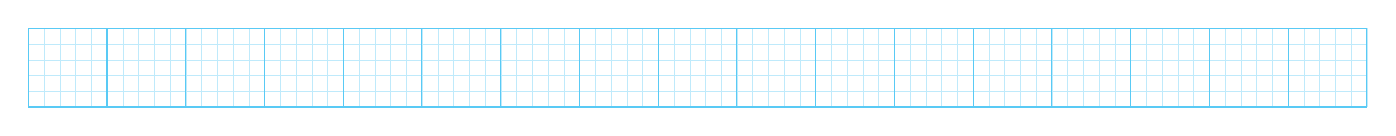
\begin{tikzpicture}
				\draw[cyan!25,ultra thin,step=0.2] (0,0) grid +(17,\myresult);
				\draw[cyan!65] (0,0) grid +(17,\myresult);
			\end{tikzpicture}
		\end{center}
	\else
	\noindent%
		\begin{center}
			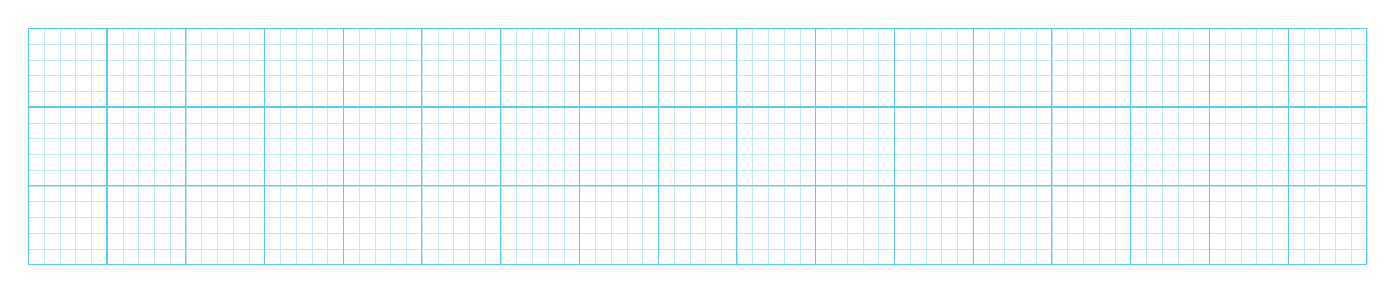
\begin{tikzpicture}
				\draw[cyan!25,ultra thin,step=0.2] (0,0) grid +(17,3);
				\draw[cyan!65] (0,0) grid +(17,3);
			\end{tikzpicture}
		\end{center}
	\fi
}

\newcommand{\DoiThanhDongKe}[1]{
\setbox0=\vbox{\hbox{
\noindent\begin{minipage}{\linewidth}%
#1 aaaaa
\end{minipage}
}}
\linepar=\ht0
\pgfmathparse{int((\linepar-\fboxsep)/(\lineheight)+1)}
	\ifnum\pgfmathresult>3
	\noindent%
		\Pointilles{\pgfmathresult}
	\else
	\noindent%
		\Pointilles{3}
	\fi
}

\newcommand{\DoiThanhDongKeH}[1]{
\setbox0=\vbox{\hbox{
\noindent\begin{minipage}{\linewidth}%
#1 aaaaa
\end{minipage}
}}
\linepar=\ht0
\pgfmathparse{int((\linepar-\fboxsep)/(0.85\lineheight)+1)}
	\ifnum\pgfmathresult>3
	\noindent%
		\Pointilles{\pgfmathresult}
	\else
	\noindent%
		\Pointilles{4}
	\fi
}
%%%=============================================%%%
\def\dongkeex{
	\AtBeginEnvironment{ex}{
		\renewcommand{\loigiai}[1]{%
		 \DoiThanhDongKe{##1}
		}
	}
	\AtBeginEnvironment{exsao}{
		\renewcommand{\loigiai}[1]{%
		 \DoiThanhDongKe{##1}
		}
	}	
}

%%%=============================================%%%
\def\Olyex{
	\AtBeginEnvironment{ex}{
		\renewcommand{\loigiai}[1]{%
			 \DoiThanhOly{##1}
		}
	}
	\AtBeginEnvironment{exsao}{
		\renewcommand{\loigiai}[1]{%
			 \DoiThanhOly{##1}
		}
	}
}

%%%=============================================%%%
\def\dongkeHaicotex{
	\AtBeginEnvironment{ex}{
		\renewcommand{\loigiai}[1]{
			\begin{multicols}{2}			
				\DoiThanhDongKeH{##1}
			\end{multicols}
		}
	}
	\AtBeginEnvironment{exsao}{
		\renewcommand{\loigiai}[1]{
			\begin{multicols}{2}			
				\DoiThanhDongKeH{##1}
			\end{multicols}
		}
	}	
}

%%%=============================================%%%
\def\tatloigiaiex{%
	\AtBeginEnvironment{ex}{\renewcommand{\loigiai}[1]{}}
	\AtBeginEnvironment{exsao}{\renewcommand{\loigiai}[1]{}}
}

%%%=============================================%%%
\def\hienthiloigiaiex{%
	\AtBeginEnvironment{ex}{
	\renewcommand{\loigiai}[1]{%
	\par\noindent%
	{\color{\maunhan}\reflectbox{\Large\WritingHand}\ {\fmmfamily\LARGE Hướng dẫn}} \faKey\ \circlenum{\Alph{numTrue}} ##1
	}
	}
	\AtBeginEnvironment{exsao}{
	\renewcommand{\loigiai}[1]{%
	\par\noindent%
	{\color{\maunhan}\reflectbox{\Large\WritingHand}\ {\fmmfamily\LARGE Hướng dẫn}} \faKey\ \circlenum{\Alph{numTrue}} ##1
	}
	}
}

%%%=============================================%%%
\def\dongkebt{
	\AtBeginEnvironment{bt}{
		\renewcommand{\loigiai}[1]{
	 \DoiThanhDongKe{##1}
		}
	}
	\AtBeginEnvironment{btsao}{
		\renewcommand{\loigiai}[1]{
	 \DoiThanhDongKe{##1}
		}
	}
}

%%%=============================================%%%
\def\Olybt{
	\AtBeginEnvironment{bt}{
		\renewcommand{\loigiai}[1]{
	 \DoiThanhOly{##1}
		}
	}
	\AtBeginEnvironment{btsao}{
		\renewcommand{\loigiai}[1]{
	 \DoiThanhOly{##1}
		}
	}
}
%%%=============================================%%%
\def\dongkeHaicotbt{
	\AtBeginEnvironment{bt}{
		\renewcommand{\loigiai}[1]{
			\begin{multicols}{2}			
				\DoiThanhDongKeH{##1}
			\end{multicols}
		}
	}
	\AtBeginEnvironment{btsao}{
		\renewcommand{\loigiai}[1]{
			\begin{multicols}{2}			
				\DoiThanhDongKeH{##1}
			\end{multicols}
		}
	}
}

%%%=============================================%%%
\def\tatloigiaibt{%
	\AtBeginEnvironment{bt}{\renewcommand{\loigiai}[1]{}}
	\AtBeginEnvironment{btsao}{\renewcommand{\loigiai}[1]{}}
}

%%%=============================================%%%
\def\hienthiloigiaibt{%
	\AtBeginEnvironment{bt}{
	\renewcommand{\loigiai}[1]{%
	\par\noindent%
	{\color{\maunhan}\reflectbox{\Large\WritingHand}\ {\fmmfamily\LARGE Hướng dẫn}} ##1
	}
	}
	\AtBeginEnvironment{btsao}{
	\renewcommand{\loigiai}[1]{%
	\par\noindent%
	{\color{\maunhan}\reflectbox{\Large\WritingHand}\ {\fmmfamily\LARGE Hướng dẫn}} ##1
	}
	}
}
\newcommand{\taoNdongke}[2][5]{
	\AtBeginEnvironment{#2}{
		\renewcommand{\loigiai}[1]{%
			\gdef\tieudehinh{}
			\Pointilles{#1}
		}
	}
	
}
%%%=========================================%%%
\Newassociation{giaibt}{loigiaibt}{ansbt}
\def\luuloigiaibt{
	\AtBeginEnvironment{bt}{
		\renewcommand{\loigiai}[1]{%
		 \scantokens{%
		 \begin{giaibt}
		 ##1
		 \end{giaibt}}
		}
	}
	\AtBeginEnvironment{btsao}{
		\renewcommand{\loigiai}[1]{%
		 \scantokens{%
		 \begin{giaibt}
		 ##1
		 \end{giaibt}}
		}
	}
}

\NewTColorBox{ansbt}{m}{
	 breakable,
	 enhanced,
	 outer arc=0pt,
	 arc=0pt,
	 colframe=white,
	 frame hidden,
	 left=-6pt,right=0pt,top=0pt,
	 colback=white,
	 attach boxed title to top left,
	 boxed title style={
	 colback=white,
	 outer arc=0pt,
	 arc=0pt,
	 top=1pt,
	 bottom=1pt,
	 left=3pt,
	 right=3pt,
	 colframe=white
 },
 fonttitle=\bfseries\sffamily\selectfont\color{white},
 title={HDBT~#1},
 overlay unbroken and first={
 \path (title.north west) coordinate (A)
 ($ (title.south west) +(-4pt,0pt)$) coordinate (B)
 (title.south east) coordinate (C)
 ($ (title.north east)+(4pt,0) $) coordinate (D);
 \path[rounded corners=2pt,fill=\mauchinh,
 preaction={transform canvas={shift={(-45:2pt)}},left color=\mauchinh!45,right color=\mauchinh!25}] 
 (A)--(B)--(C)--(D)--cycle;
 \path (A)--(C) node[midway,font=\color{white}\bfseries\sffamily\selectfont](Bai){\textsl{HDBT~#1}};
 \draw[rounded corners=2pt,thick,\mauchinh] ([xshift=-3pt]B) coordinate (Bt)
 --([shift={(-2pt,2pt)}]A)--+(\linewidth,0) coordinate (Ct);
 \fill[\mauchinh] (Bt) circle (1pt) (Ct) circle (2pt);
}
}

\renewenvironment{loigiaibt}[1]{\begin{ansbt}{#1}}{\end{ansbt}}

%%%=============================================%%%
\def\dongkevd{
	\AtBeginEnvironment{vd}{
		\renewcommand{\loigiai}[1]{%
			\end{boxvd}\def\vdend{}
	 \DoiThanhDongKe{##1}
		}
	}
}

%%%=============================================%%%
\def\Olyvd{
	\AtBeginEnvironment{vd}{
		\renewcommand{\loigiai}[1]{
	 \DoiThanhOly{##1}
		}
	}
}

%%%=============================================%%%
\def\dongkeHaicotvd{
	\AtBeginEnvironment{vd}{
		\renewcommand{\loigiai}[1]{%
			\end{boxvd}\def\vdend{}
				\begin{multicols}{2}			
					\DoiThanhDongKeH{##1}
				\end{multicols}
		}
	}
}

%%%=============================================%%%
\def\tatloigiaivd{
	\AtBeginEnvironment{vd}{
		\renewcommand{\loigiai}[1]{}%
	}
}

\def\hienthiloigiaivd{
\AtBeginEnvironment{vd}{
	\renewcommand{\loigiai}[1]{
		\end{boxvd}
		\def\vdend{}
			\par\noindent{\color{\maunhan}\reflectbox{\Large\WritingHand}\ {\fmmfamily\LARGE Lời giải.}}
		##1
		}
	}
}

%%%======================================================%%%
\newcommand{\taosao}[1]{%
\ifcase#1\relax%
 \or
 \faStar~\faStarO~\faStarO~\faStarO~\faStarO
 \or
 \faStar~\faStar~\faStarO~\faStarO~\faStarO
 \or
 \faStar~\faStar~\faStar~\faStarO~\faStarO
 \or
 \faStar~\faStar~\faStar~\faStar~\faStarO
 \else
 \faStar~\faStar~\faStar~\faStar~\faStar
 \fi
}



\NewTColorBox{ext}{+!O{}O{}}{
	 breakable,
	 enhanced,
	 outer arc=0pt,
	 arc=0pt,
	 colframe=white,
	 frame hidden,
	 left=-6pt,right=0pt,top=0pt,
	 colback=white,
	 attach boxed title to top left,
 boxed title style={
	 colback=white,
	 outer arc=0pt,
	 arc=0pt,
	 top=1pt,
	 bottom=1pt,
	 left=3pt,
	 right=3pt,
	 colframe=white
 },
 fonttitle=\bfseries\fontfamily{pag}\selectfont\color{white},
 title={Câu~\theex},
 overlay unbroken and first={
	 \path
		 ($ (title.north west) +(-9pt,0pt)$) coordinate (A)
		 ($ (title.south west) +(-15pt,0pt)$) coordinate (B)
		 (title.south east) coordinate (C)
		 ($ (title.north east)+(-5pt,0) $) coordinate (D);
		 \path[left color=\maudam, right color=\maudam!65]
		 ([shift={(-4.5pt,0pt)}]A)--+(4.5pt,0)--([turn]-115:13pt)--([turn]-65:4.5pt)--cycle;
		 %Dậm ở dưới
		 \path[left color=\maudam, right color=\maudam!65!white!65]
		 ([shift={(5pt,3pt)}]A)--+(29pt,0) coordinate (Am) --([turn]-115:21pt)--([turn]-65:29pt)--cycle; 
		 %Thanh dọc lớn
		 \path[left color=\maudam,right color=\maudam!75]
		 ([shift={(5pt,7pt)}]A)--+(7pt,0)--([turn]-115:31pt)--([turn]-65:7pt)--cycle; 
		 %Tanh doc lớn
		 \path[fill=\mautuongdong!75] let \p1=($(D) - (A) $) in 
		 (Am)--+({veclen(\x1,\y1)},0) coordinate (Ah) --([turn]-115:21pt)--([turn]-65:{veclen(\x1,\y1)})--cycle; 
		 %Thanh dọc dài
		 \begin{pgfonlayer}{background}
		 \path[left color=\mautuongdong!75,right color=\mautuongdong!45]
		 ([shift={(-5pt,-7pt)}]Ah)--+(0.865\linewidth,0) coordinate (Ab) --([turn]-115:7pt)--([turn]-65:0.865\linewidth) --cycle;
		 \end{pgfonlayer}
		 
		\path ([shift={(0.65pt,-0.7pt)}]Am) node[anchor=north west,font=\color{gray!85!black}\bfseries\sffamily\selectfont]{{Câu~\theex}};
		 
		\path (Am) node[anchor=north west,font=\color{white}\bfseries\sffamily\selectfont]{{Câu~\theex}};
	
		\ifblank{#2}{%
			\path (Ab) node[anchor=south east,font=\color{\maudam!65}\scriptsize,inner sep=1pt]{\taosao{1}};
		}{%
			\path (Ab) node[anchor=south east,font=\color{\maudam!65}\scriptsize,inner sep=1pt]{\taosao{#2}};
		}
	 
	 \ifblank{#1}{}{%
	 \path ($(Ah)+(-1pt,-13pt)$) node[anchor=south west,font=\footnotesize\sffamily,text=\maudam!95!black]{\textit{Nguồn: #1}};
	 }
	 
		\path ([shift={(-6pt,-1pt)}]Am) node[anchor=north east,font=\color{white}]{\faGg};
 },
 lowerbox=ignored
}
 
\newcommand{\exhead}[2]{\begin{ext}[#1][#2]}
\newcommand{\exend}{\end{ext}}
\NewDocumentEnvironment{exsao}{+!O{}O{}}{\exhead{#1}{#2}}{\exend}
 
\AtBeginEnvironment{exsao}{
 \refstepcounter{ex}
 \setcounter{numTrue}{0}%
 \setcounter{numTrueSol}{0}%
 \renewcommand{\loigiai}[1]{\par\noindent%
 {\color{\mautuongdong}\reflectbox{\Large\WritingHand}\ {\fmmfamily\LARGE Lời giải.}} #1
 \ifthenelse{\value{numTrueSol}>0}{
 \hfill \textcolor{\mautuongdong}{\sffamily \faKey~\circlenum{\Alph{numTrueSol}}}
 }{}
 }
} 

\NewTColorBox{btsao}{+!O{}O{}}{
 breakable,
 enhanced,
 outer arc=0pt,
 arc=0pt,
 colframe=white,
 frame hidden,
 left=-3pt,right=0pt,top=0pt,
 colback=white,
 attach boxed title to top left,
 boxed title style={
	 colback=white,
	 outer arc=0pt,
	 arc=0pt,
	 top=1pt,
	 bottom=1pt,
	 left=3pt,
	 right=3pt,
	 colframe=white
 },
 fonttitle=\bfseries\sffamily\selectfont\color{white},
 title={Bài~\thebt},
 overlay unbroken and first={
 \path
 (title.north west) coordinate (A)
 ($ (title.south west) +(-4pt,0pt)$) coordinate (B)
 (title.south east) coordinate (C)
 ($ (title.north east)+(4pt,0) $) coordinate (D);
 
 \path[rounded corners=2pt,fill=\mauchinh,
 preaction={transform canvas={shift={(-45:2pt)}},left color=\mauchinh!45,right color=\mauchinh!25}] 
 (A)--(B)--(C)--(D)--cycle;
 \path (A)--(C) node[midway,font=\color{white}\bfseries\fontfamily{pag}\selectfont](Bai){\textsl{Bài~\thebt}};
 \draw[rounded corners=2pt,thick,\mauchinh] ([xshift=-3pt]B) coordinate (Bt)
 --([shift={(-2pt,2pt)}]A)--+(\linewidth,0) coordinate (Ct);
 \fill[\mauchinh] (Bt) circle (1pt) (Ct) circle (2pt);

 \ifblank{#2}{\path ([shift={(0,-9pt)}]Ct) node[anchor=east,font=\color{\maunhan}]{{\starlet\ }};}%
 {\path ([shift={(0,-9pt)}]Ct) node[anchor=east,font=\color{\maunhan}]{\foreach \i in {1,...,#2}{\starlet\ }};} 
 \ifblank{#1}{}{\path ($ (D)!0.5!(C) $) node[anchor=west,font=\color{\mauchinh},text width=0.5\linewidth]{(\textsf{#1})}; }
 }
}

\AtBeginEnvironment{btsao}{
 \refstepcounter{bt}
 \renewcommand{\loigiai}[1]{\par\noindent%
 {\color{\maunhan}\reflectbox{\Large\WritingHand}\ {\fmmfamily\LARGE Hướng dẫn.}} #1}
} 

\NewTColorBox{boxvdsao}{+!O{}O{}}{
	enhanced,
	fonttitle=\bfseries\sffamily\color{white},
	title={\faGg\ Ví dụ~\thevd a},
	colframe=white,
	colback=white,
	colbacktitle=white,
	fonttitle=\bfseries,
	coltitle=black,
	boxsep=0pt,
	attach boxed title to top left=
	{yshift=-2mm-\tcboxedtitleheight,yshifttext=2mm-\tcboxedtitleheight/2},
	boxed title style={
	frame hidden,
	outer arc=0pt,
	arc=0pt,
	top=3pt,
	bottom=3pt,
	left=0pt,
	right=0pt
},
overlay unbroken and first={
	\path
	($ (title.north west) +(-2pt,0pt)$) coordinate (A)
	($ (title.south west) +(-2pt,3pt)$) coordinate (B)
	($ (title.south east)+(3pt,3pt) $) coordinate (C)
	($ (title.north east)+(3pt,0) $) coordinate (D)
	(intersection of C--B and frame.north east--frame.south east) coordinate (Et)
	(intersection of A--D and frame.north east--frame.south east) coordinate (Ft)
	($ (Et)-(4pt,0) $) coordinate (E)
	($(Ft)-(4pt,0)$) coordinate (F);
\draw[line width=1.65pt,gray!25,rounded corners=3pt] ($ (frame.north west) +(0,-2pt)$) rectangle (frame.south east);
\path[fill=\mycolor!25,rounded corners=3pt]
(A)--(B)--(E)--(F)--cycle;
\path[fill=\mycolor!70!black,rounded corners=2pt]
(A)--(B)--([xshift=3pt]C)--([xshift=3pt]D)--cycle;
\path[left color=\mycolor,right color=\mycolor!80,rounded corners=3pt]
([xshift=-2pt]A)--([xshift=-2pt]B)--(C)--(D)--cycle;

\path ($ (A)!0.5!(B) +(9pt,0)$) node[anchor=west,font=\color{white}\bfseries\sffamily\selectfont]{{\faGg\ Ví dụ~\thevd}};

\path ($ (C)!0.5!(D) +(3pt,0)$) node[anchor=west,font=\color{\mycolor!70!black}\fontfamily{pag}\selectfont\footnotesize]{#1};

\ifblank{#2}{%
	\path ($ (E)!0.5!(F) +(-5pt,0)$) node[anchor=east,font=\color{\mycolor}]{\taosao{1}};
	}{%
	\path ($ (E)!0.5!(F) +(-5pt,0)$) node[anchor=east,font=\color{\mycolor}]{\taosao{#2}};
	},
},
top=\tcboxedtitleheight
}
\newcommand{\vdsaohead}[2]{\begin{boxvdsao}[#1][#2]}

\newcommand{\vdsaoend}{\end{boxvdsao}}
\NewDocumentEnvironment{vdsao}{+!O{}O{}}{\vdsaohead{#1}{#2}}{\vdsaoend}

\AtBeginEnvironment{vdsao}{
 \refstepcounter{vd}%
 \setcounter{numTrue}{0}%
 \setcounter{numTrueSol}{0}%
 \renewcommand{\loigiai}[1]{\par\noindent%
 {\color{\mycolor}\reflectbox{\Large\WritingHand}\ {\fmmfamily\LARGE Lời giải.}} #1}
}